% ============================================================
%  WaveLabX -- Software Architecture diagram (manuscript Figure 1)
%  Lamsal & Rhode-Barbarigos (2026)
%  Compile:  pdflatex wavelabx_architecture.tex
%  Full-page-width figure; every text node has a fixed text width
%  so content wraps and never overflows its box.
% ============================================================
\documentclass[border={0pt 6pt 6pt 6pt}]{standalone}
\usepackage{tikz}
\usepackage{amsmath}
\usepackage{lmodern}
\usetikzlibrary{positioning, arrows.meta, shapes.geometric, fit, calc}

%% ---- Colour palette --------------------------------------------------------
\definecolor{wlxBlue}{RGB}{33,94,168}
\definecolor{wlxBlueLt}{RGB}{233,241,251}
\definecolor{wlxViolet}{RGB}{94,80,162}
\definecolor{wlxVioletLt}{RGB}{240,237,249}
\definecolor{wlxOrange}{RGB}{190,112,40}
\definecolor{wlxOrangeLt}{RGB}{253,241,225}
\definecolor{wlxRed}{RGB}{182,60,56}
\definecolor{wlxRedLt}{RGB}{252,234,232}
\definecolor{wlxTeal}{RGB}{19,118,98}
\definecolor{wlxTealLt}{RGB}{228,244,240}
\definecolor{wlxTealDk}{RGB}{11,74,61}
\definecolor{wlxGray}{RGB}{110,110,110}
\definecolor{wlxBorder}{RGB}{172,172,172}
\definecolor{wlxInk}{RGB}{42,42,42}

\begin{document}
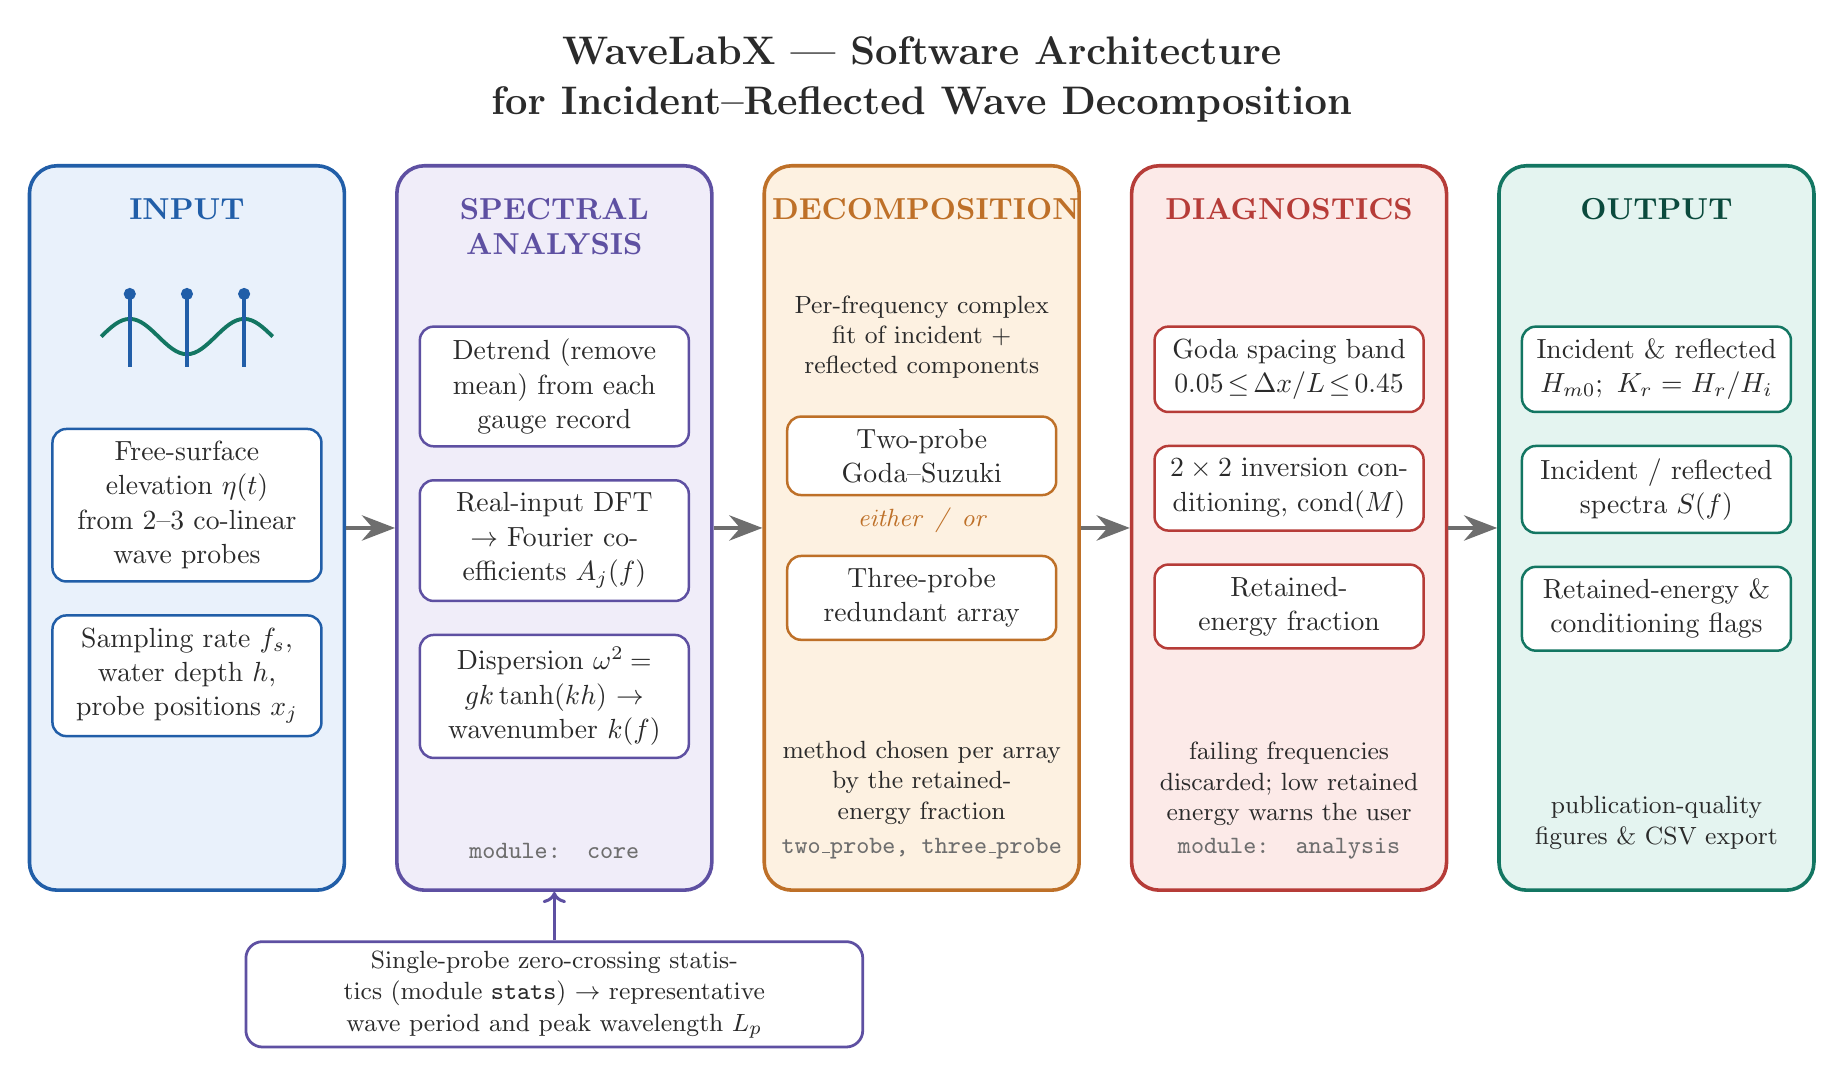
\begin{tikzpicture}[
  font=\sffamily,
  block/.style   = {rectangle, rounded corners=10pt, line width=1.3pt,
                    minimum width=4.0cm, minimum height=9.2cm},
  inblk/.style   = {block, draw=wlxBlue,   fill=wlxBlueLt},
  preblk/.style  = {block, draw=wlxViolet, fill=wlxVioletLt},
  decblk/.style  = {block, draw=wlxOrange, fill=wlxOrangeLt},
  diagblk/.style = {block, draw=wlxRed,    fill=wlxRedLt},
  outblk/.style  = {block, draw=wlxTeal,   fill=wlxTealLt},
  btitle/.style  = {text width=3.8cm, align=center,
                    font=\fontsize{10.5}{12.5}\bfseries\selectfont},
  sub/.style     = {rectangle, rounded corners=5pt, line width=0.9pt,
                    fill=white, text width=3.1cm, align=center,
                    inner sep=4.5pt, text=wlxInk,
                    font=\fontsize{10.4}{12.4}\selectfont},
  bsub/.style    = {sub, draw=wlxBlue},
  psub/.style    = {sub, draw=wlxViolet},
  dsub/.style    = {sub, draw=wlxOrange},
  gsub/.style    = {sub, draw=wlxRed},
  osub/.style    = {sub, draw=wlxTeal},
  note/.style    = {text width=3.55cm, align=center, text=wlxInk,
                    font=\fontsize{9}{11}\selectfont},
  mtag/.style    = {font=\ttfamily\fontsize{8.6}{10}\selectfont,
                    text=wlxGray},
  arrow/.style   = {-{Stealth[length=4.2mm,width=3.2mm]}, line width=1.6pt,
                    color=wlxGray},
]

% ===================== BLOCK 1 -- INPUT ===================================
\node[inblk] (input) at (0,0) {};
\node[btitle, text=wlxBlue, anchor=north] at ($(input.north)+(0,-0.32)$)
  {INPUT};
\node[anchor=north] at ($(input.north)+(0,-1.45)$){%
  \tikz[scale=0.66]{%
    \draw[wlxTeal, line width=1.4pt]
      (0,0) sin (0.55,0.34) cos (1.1,0) sin (1.65,-0.34) cos (2.2,0)
            sin (2.75,0.34) cos (3.3,0);
    \foreach \x in {0.55,1.65,2.75}{%
      \draw[wlxBlue, line width=1.4pt] (\x,-0.58) -- (\x,0.82);
      \filldraw[wlxBlue] (\x,0.82) circle (3pt);}}};
\node[bsub, anchor=north] (i1) at ($(input.north)+(0,-3.35)$)
  {Free-surface elevation $\eta(t)$ from 2--3 co-linear wave probes};
\node[bsub, anchor=north] (i2) at ($(i1.south)+(0,-0.40)$)
  {Sampling rate $f_s$, water depth $h$, probe positions $x_j$};

% ===================== BLOCK 2 -- SPECTRAL ANALYSIS =======================
\node[preblk, right=0.62cm of input] (pre) {};
\node[btitle, text=wlxViolet, anchor=north] at ($(pre.north)+(0,-0.32)$)
  {SPECTRAL\\ANALYSIS};
\node[psub, anchor=north] (s1) at ($(pre.north)+(0,-2.05)$)
  {Detrend (remove mean) from each gauge record};
\node[psub, anchor=north] (s2) at ($(s1.south)+(0,-0.40)$)
  {Real-input DFT $\rightarrow$ Fourier coefficients $A_j(f)$};
\node[psub, anchor=north] (s3) at ($(s2.south)+(0,-0.40)$)
  {Dispersion $\omega^2\!=\!g k\tanh(kh)$ $\rightarrow$ wavenumber $k(f)$};
\node[mtag, anchor=south] at ($(pre.south)+(0,0.30)$) {module: core};

% ===================== BLOCK 3 -- DECOMPOSITION ===========================
\node[decblk, right=0.62cm of pre] (dec) {};
\node[btitle, text=wlxOrange, anchor=north] at ($(dec.north)+(0,-0.32)$)
  {DECOMPOSITION};
\node[note, anchor=north] (df) at ($(dec.north)+(0,-1.55)$)
  {Per-frequency complex fit of incident $+$ reflected components};
\node[dsub, anchor=north] (d1) at ($(df.south)+(0,-0.34)$)
  {Two-probe\\Goda--Suzuki};
\node[font=\fontsize{9.2}{10}\itshape\selectfont, text=wlxOrange]
  (eor) at ($(d1.south)+(0,-0.30)$) {either\, /\, or};
\node[dsub, anchor=north] (d2) at ($(eor.south)+(0,-0.16)$)
  {Three-probe\\redundant array};
\node[note, anchor=south] at ($(dec.south)+(0,0.74)$)
  {method chosen per array by the retained-energy fraction};
\node[mtag, anchor=south] at ($(dec.south)+(0,0.30)$)
  {two\_probe, three\_probe};

% ===================== BLOCK 4 -- DIAGNOSTICS =============================
\node[diagblk, right=0.62cm of dec] (diag) {};
\node[btitle, text=wlxRed, anchor=north] at ($(diag.north)+(0,-0.32)$)
  {DIAGNOSTICS};
\node[gsub, anchor=north] (g1) at ($(diag.north)+(0,-2.05)$)
  {Goda spacing band $0.05\!\le\!\Delta x/L\!\le\!0.45$};
\node[gsub, anchor=north] (g2) at ($(g1.south)+(0,-0.40)$)
  {$2\times2$ inversion conditioning, $\mathrm{cond}(M)$};
\node[gsub, anchor=north] (g3) at ($(g2.south)+(0,-0.40)$)
  {Retained-energy fraction};
\node[note, anchor=south] at ($(diag.south)+(0,0.72)$)
  {failing frequencies discarded; low retained energy warns the user};
\node[mtag, anchor=south] at ($(diag.south)+(0,0.30)$) {module: analysis};

% ===================== BLOCK 5 -- OUTPUT ==================================
\node[outblk, right=0.62cm of diag] (out) {};
\node[btitle, text=wlxTealDk, anchor=north] at ($(out.north)+(0,-0.32)$)
  {OUTPUT};
\node[osub, anchor=north] (o1) at ($(out.north)+(0,-2.05)$)
  {Incident \& reflected $H_{m0}$;\, $K_r = H_r/H_i$};
\node[osub, anchor=north] (o2) at ($(o1.south)+(0,-0.40)$)
  {Incident / reflected spectra $S(f)$};
\node[osub, anchor=north] (o3) at ($(o2.south)+(0,-0.40)$)
  {Retained-energy \& conditioning flags};
\node[note, anchor=south] at ($(out.south)+(0,0.42)$)
  {publication-quality figures \& CSV export};

% ===================== PIPELINE ARROWS ====================================
\draw[arrow] (input.east) -- (pre.west);
\draw[arrow] (pre.east)   -- (dec.west);
\draw[arrow] (dec.east)   -- (diag.west);
\draw[arrow] (diag.east)  -- (out.west);

% ===================== ZERO-CROSSING FEEDER ===============================
\node[rectangle, rounded corners=6pt, draw=wlxViolet, line width=1pt,
      fill=white, text width=7.6cm, align=center, text=wlxInk,
      font=\fontsize{9.4}{11.4}\selectfont] (zc)
      at ($(pre.south)+(0,-1.30)$)
  {Single-probe zero-crossing statistics (module \texttt{stats})
   $\rightarrow$ representative wave period and peak wavelength $L_p$};
\draw[->, line width=1.1pt, wlxViolet] (zc.north) -- (zc.north|-pre.south);

% ===================== TITLE ==============================================
\node[fit=(input)(pre)(dec)(diag)(out), inner sep=0pt] (arch) {};
\node[font=\fontsize{15}{18}\bfseries\selectfont, text=wlxInk,
      anchor=south, align=center, text width=22cm]
      at ($(arch.north)+(0,0.4)$)
  {WaveLabX --- Software Architecture\\
   for Incident--Reflected Wave Decomposition};

\end{tikzpicture}
\end{document}
